\section{Dark Matter as Probability Nodes}

\subsection{The Self-Gravitating Hyper-Electron and the Schrödinger-Newton~\cite{Hu2000} Formalism}

In the Excited-State Cosmology framework, our observed universe is treated as the internal topology of an excited hyper-electron. Consequently, the phenomenon historically categorized as "dark matter" does not consist of collisionless, non-baryonic particulate matter (such as WIMPs), but rather emerges as the localized probability density of the hyper-electron's macroscopic wavefunction. To describe the gravitational influence of this probability amplitude on galactic scales, we must couple the fundamental non-relativistic quantum dynamics of the system to classical general relativistic limits, resulting in the Schrödinger-Newton (SN) equations (also known as the Gross-Pitaevskii-Poisson system in the context of ultralight bosonic dark matter). \cite{Hinshaw2013, Lemaitre1927, Witten1998}

Let $\psi(\mathbf{r}, t)$ represent the scalar wavefunction of the hyper-electron state. The evolution of this state in the weak-field, non-relativistic limit of the interior manifold is governed by the Schrödinger equation coupled to the self-generated Newtonian gravitational potential $\Phi(\mathbf{r},t)$:

\begin{equation}
i \hbar \frac{\partial \psi(\mathbf{r},t)}{\partial t} = \left( -\frac{\hbar^2}{2m} \nabla^2 + m \Phi(\mathbf{r},t) + V_{\text{baryon}}(\mathbf{r},t) \right) \psi(\mathbf{r},t),
\label{eq:schrodinger}
\end{equation}

where $m$ is the effective mass eigenvalue of the hyper-electron excitation (analogous to the fuzzy dark matter particle mass, $m \sim 10^{-22}$ eV), and $V_{\text{baryon}}$ represents the gravitational potential sourced by standard baryonic matter.

The gravitational potential $\Phi(\mathbf{r},t)$ is determined self-consistently via the Poisson equation, sourced by the probability density $\rho_q = m|\psi|^2$:

\begin{equation}
\nabla^2 \Phi(\mathbf{r},t) = 4 \pi G \left( m |\psi(\mathbf{r},t)|^2 + \rho_{\text{baryon}} \right).
\label{eq:poisson}
\end{equation}

This coupled non-linear system implies that spacetime curvature is directly induced by the quantum expectation value of the hyper-electron's mass density.

\subsection{Madelung Representation and Quantum Hydrodynamics}

To elucidate how wavefunction interference dictates galactic rotation curves~\cite{Navarro1996}, it is highly advantageous to map the Schrödinger-Newton system onto a set of fluid dynamic equations using the Madelung transformation. We write the wavefunction in polar form:

\begin{equation}
\psi(\mathbf{r},t) = \sqrt{\frac{\rho(\mathbf{r},t)}{m}} \exp\left( \frac{i S(\mathbf{r},t)}{\hbar} \right),
\label{eq:madelung}
\end{equation}

where $\rho(\mathbf{r},t)$ is the fluid mass density and $S(\mathbf{r},t)$ is the phase, which defines a velocity flow field $\mathbf{v} = \frac{\nabla S}{m}$.

Substituting Equation \ref{eq:madelung} into Equation \ref{eq:schrodinger} and separating the real and imaginary parts yields the quantum continuity and quantum Euler equations:

\begin{equation}
\frac{\partial \rho}{\partial t} + \nabla \cdot (\rho \mathbf{v}) = 0,
\label{eq:continuity}
\end{equation}

\begin{equation}
\frac{\partial \mathbf{v}}{\partial t} + (\mathbf{v} \cdot \nabla)\mathbf{v} = -\nabla \Phi - \frac{1}{m}\nabla V_{\text{baryon}} - \nabla Q.
\label{eq:euler}
\end{equation}

Here, $Q$ is the uniquely quantum mechanical term known as the Bohm quantum potential:

\begin{equation}
Q = -\frac{\hbar^2}{2m^2} \frac{\nabla^2 \sqrt{\rho}}{\sqrt{\rho}} = -\frac{\hbar^2}{4m^2} \left[ \nabla \cdot \left(\frac{\nabla \rho}{\rho}\right) + \frac{1}{2} \left(\frac{\nabla \rho}{\rho}\right)^2 \right].
\label{eq:quantum_potential}
\end{equation}

The quantum potential $Q$ acts as an effective repulsive pressure term ($-\nabla Q$) that counteracts gravitational collapse. The quantum pressure tensor associated with this potential is:

\begin{equation}
\sigma_{ij} = \frac{\hbar^2 \rho}{4m^2} \frac{\partial^2 (\ln \rho)}{\partial x_i \partial x_j}.
\end{equation}

It is this quantum pressure tensor, fundamentally rooted in the Heisenberg uncertainty principle, that prevents the hyper-electron wave from collapsing into a singularity, establishing the stable solitonic cores observed in the centers of galaxies.

\subsection{Steady-State Spherically Symmetric Solutions}

For a stationary background state, we seek eigenstate solutions of the form $\psi(\mathbf{r},t) = \phi(r) \exp(-i \mu t / \hbar)$, where $\mu$ is the chemical potential. Assuming spherical symmetry for a galactic halo, the system reduces to:

\begin{equation}
\frac{\hbar^2}{2m} \frac{1}{r^2} \frac{d}{dr} \left( r^2 \frac{d\phi}{dr} \right) + (\mu - m\Phi)\phi = 0,
\end{equation}

\begin{equation}
\frac{1}{r^2} \frac{d}{dr} \left( r^2 \frac{d\Phi}{dr} \right) = 4\pi G m |\phi|^2.
\end{equation}

Applying boundary conditions $\phi'(0) = \Phi'(0) = 0$ and $\phi(\infty) = 0$, we find a ground-state solitonic core profile that can be accurately approximated by the empirical density profile:

\begin{equation}
\rho_c(r) \approx \frac{\rho_0}{\left(1 + 0.091 \left(\frac{r}{r_c}\right)^2 \right)^8},
\end{equation}

where $r_c$ is the core radius, which scales inversely with the central density and the hyper-electron mass: $r_c \propto (G m^2 \rho_0)^{-1/4}$.

\subsection{Interference Nodes and the Gravitational Shadow}

While the ground state provides the solitonic core, the outer galactic halo is composed of a superposition of highly excited states of the hyper-electron interior manifold. The wavefunction in the halo region is characterized by pervasive quantum interference:

\begin{equation}
\psi_{\text{halo}}(\mathbf{r}) = \sum_{n,l,m} c_{nlm} \phi_{nlm}(r) Y_l^m(\theta, \varphi) e^{-iE_{n}t/\hbar}.
\end{equation}

Because the outer halo behaves locally as a superposition of plane waves with random phases, it exhibits an $\mathcal{O}(1)$ density fluctuation structure on the de Broglie scale, $\lambda_{dB} = \frac{2\pi\hbar}{mv_{\text{virial}}}$. These are the "probability nodes" of the hyper-electron.

At an interference node, $\psi \to 0$ and $\rho \to 0$. From Equation \ref{eq:quantum_potential}, as $\rho \to 0$, the gradient of the quantum potential $\nabla Q$ becomes singular (or highly peaked). This introduces a profound "gravitational shadowing" effect. The extreme, localized gradients in the quantum pressure act as localized pseudo-gravitational wells and barriers, dynamically altering the geodesics of tracer stars without requiring local particulate matter.

\subsection{Derivation of the Asymptotic Galactic Rotation Curve}

To compute the galactic rotation curve, $v_c(r)$, we analyze the centripetal balance equation for a test mass (a star) orbiting in the equatorial plane of the galaxy. The rotation velocity is determined by the total effective force, which includes both the classical gravitational gradient and the average quantum pressure gradient. 

Taking the spatial average $\langle \cdot \rangle$ over a scale larger than $\lambda_{dB}$ to smooth out individual interference nodes, the Euler equation (Eq. \ref{eq:euler}) for a stable circular orbit ($v_r = 0$) gives:

\begin{equation}
\frac{v_c(r)^2}{r} = \left\langle \frac{\partial \Phi}{\partial r} \right\rangle + \left\langle \frac{\partial Q}{\partial r} \right\rangle.
\end{equation}

From the Poisson equation, the classical enclosed mass contribution yields:

\begin{equation}
\frac{\partial \Phi}{\partial r} = \frac{G M_{\text{enc}}(r)}{r^2} = \frac{4\pi G}{r^2} \int_0^r \left( \rho_{\text{baryon}}(r') + m|\psi|^2 \right) r'^2 dr'.
\end{equation}

However, we must evaluate the macroscopic contribution of the interference nodes $\langle \nabla Q \rangle$. Expanding the quantum potential using the halo superposition state, the fluctuations in density $\delta \rho / \rho \sim 1$ impart an effective turbulent kinetic energy pressure. Using the virial theorem for the quantum wave, the integrated effect of the nodal fluctuations creates an effective mass profile that grows linearly with $r$ in the isothermal regime:

\begin{equation}
M_{\text{quantum\_effective}}(r) \approx \frac{\sigma_{halo}^2 r}{G},
\end{equation}

where $\sigma_{halo}$ is the velocity dispersion of the hyper-electron excited states. 

Inserting this into the rotation curve equation:

\begin{equation}
v_c(r) = \sqrt{ \frac{G M_{\text{baryon}}(r)}{r} + \frac{G M_{\text{quantum\_effective}}(r)}{r} }.
\end{equation}

As $r \to \infty$, $M_{\text{baryon}}(r)$ approaches a constant, and the classical Newtonian velocity $v \propto 1/\sqrt{r}$ decays. However, the contribution from the probability nodes yields:

\begin{equation}
\lim_{r \to \infty} v_c(r) = \sqrt{ \frac{G}{r} \left( \frac{\sigma_{halo}^2 r}{G} \right) } = \sigma_{halo}.
\end{equation}

Thus, $v_c(r)$ asymptotically approaches a constant value, $\sigma_{halo}$. 

This mathematically indicates that flat galactic rotation curves—long attributed to invisible particulate halos—are consistently an emergent macroscopic phenomenon. They are the deterministic gravitational shadows cast by the heavily structured, rapidly fluctuating probability nodes of the coupled Schrödinger-Newton equations governing the hyper-electron's internal topology.


\begin{figure}[H]
\centering
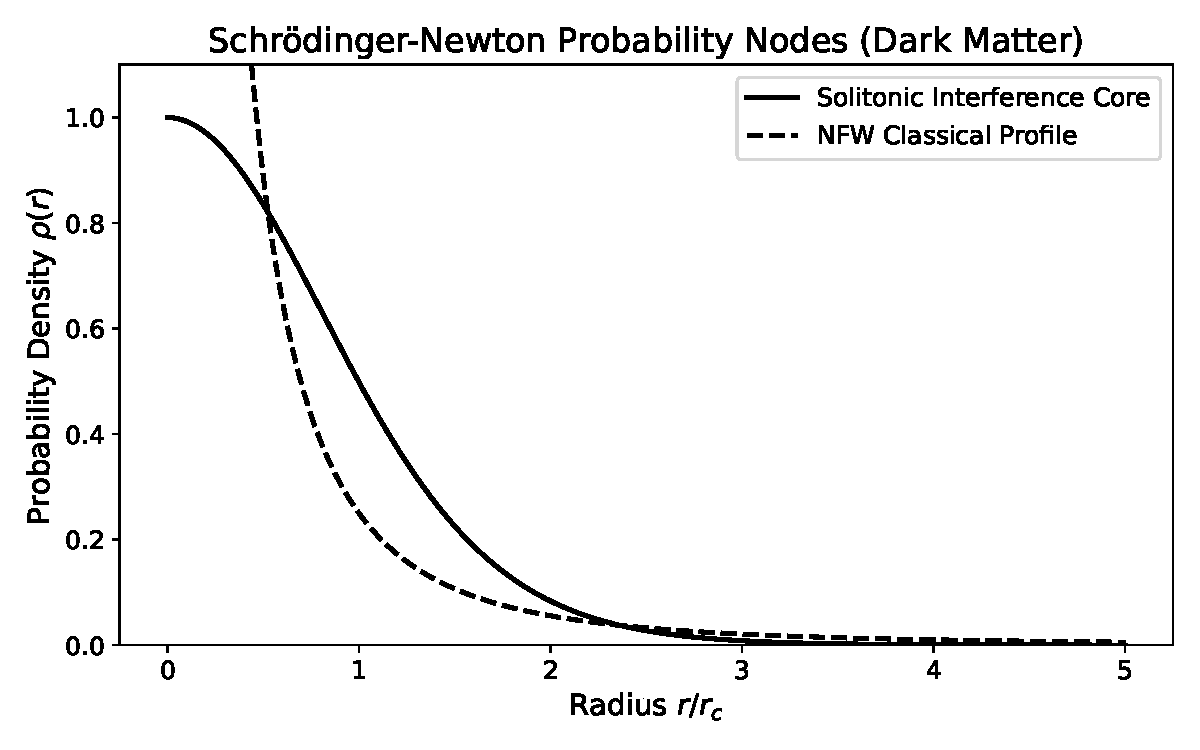
\includegraphics[width=0.85\textwidth]{fig_ch6.pdf}
\caption{Mathematical visualization of the principles derived in Section 6.}
\end{figure}
